\documentclass[aspectratio=169,xcolor=dvipsnames]{beamer}

\usepackage[utf8]{inputenc}
\usepackage[ngerman]{babel}
\usepackage[T1]{fontenc}
\usepackage{amsmath}
\usepackage{amsfonts}
\usepackage{amssymb}
\usepackage{graphicx}
\usepackage{amsthm}
\usepackage{courier}
%\usepackage[left=0.1cm,right=0.1cm,top=1cm,bottom=1cm]{geometry}
\usepackage{xcolor}
\usepackage{enumerate}
\usepackage{todonotes}
\usepackage[babel,german=quotes]{csquotes}
\usepackage[style=numeric, backend=bibtex]{biblatex}
\usepackage{tikz}
\usepackage{hyperref}
\usepackage{listings}
\usepackage{verbatim}
\usepackage{xpatch}
\usepackage{lscape}
%\usepackage{mathptmx}
\usepackage{longtable}
\usepackage{pdfpages}
\usepackage{hyperref}
\usepackage{pifont}
%\usepackage[onehalfspacing]{setspace}
\usepackage{caption}
\captionsetup{font={scriptsize}}
\usepackage{multimedia}
\usepackage{media9}
\usepackage{mathrsfs}
\usepackage{bm}

\usetheme{EastLansing}
%\usecolortheme{crane}
\usefonttheme{professionalfonts}
\useinnertheme{rounded}
\useoutertheme{default}

\newtheorem{satz}{Satz}
\newtheorem{law}{Gesetz}
\newtheorem{postulat}{Postulate}
\newtheorem{ex}{Beispiel}

\def\colorize<#1>{%
	\temporal<#1>{\color{red!50}}{\color{black}}{\color{black!50}}}
\setbeamertemplate{footline}[frame number, title, author]
\setbeamerfont{caption}{size=\scriptsize}
\setbeamerfont{footnote}{size=\scriptsize}
\setbeamercolor{item}{use={structure,normal text},fg=structure.fg!0!normal text.fg}
\setbeamercolor{special text}{use={1,0,0}}
\setbeamertemplate{navigation symbols}{\insertframenavigationsymbol\insertbackfindforwardnavigationsymbol}
\setbeamercolor{title}{fg=black!70!white,bg=green!10!yellow}
\setbeamercolor*{palette primary}{fg=green!10!yellow,bg=black!30!white}
\setbeamercolor*{palette secondary}{use=structure,fg=green!10!yellow,bg=black!50!white}
\setbeamercolor*{palette tertiary}{use=structure,fg=green!10!yellow,bg=black!70!white}
\setbeamercolor{frametitle}{fg=black!70!white,bg=green!10!yellow!70!white}
\setbeamertemplate{headline}
{%
	\begin{beamercolorbox}{section in head/foot}
		\vskip2pt\insertnavigation{\paperwidth}\vskip2pt
	\end{beamercolorbox}%
}
\setbeamercolor{block title}{fg=black!70!white,bg=green!10!yellow}
\setbeamercolor{block body}{use=structure,fg=black,bg=green!10!yellow!30!white}
\setbeamercolor{codex}{fg=black,bg=green!10!yellow!30!white}

\usepackage{remreset}
\makeatletter

\title[Bayes-Statistik \& Wahlprognosen]{\textbf{Tag 5: Bayes-Statistik und Wahlprognosen}}
\author[Philip \and Tanja \and Maximilian]{Philip Biegel \and Tanja Bien \and Maximilian Wiesmann}
\institute[]{Sommerakademie der Studienstiftung Olang - Arbeitsgruppe 4: Empirische Wahlforschung und Wahlprognosen}
\date{6. September 2019}


\begin{document}

\begin{frame}
\titlepage
\end{frame}

\begin{frame}
\frametitle{Inhalt}
\section[Inhalt]{Inhalt}
\tableofcontents
\end{frame}

\section{Bayessche Inferenz}
\begin{frame}
\frametitle{Bayessche Inferenz}
\begin{itemize}
	\item[]<1-> 
	\begin{beamercolorbox}[sep=0.5em,wd=\textwidth,shadow=true,rounded=true]{codex}
		\textit{\glqq At the heart of statistics lie the ideas of statistical inference. Methods of statistical inference enable the investigator to argue from the particular observations in a sample to the general case. In contrast to logical deductions made from the general case to the specific case, a statistical inference can sometimes be incorrect. Nevertheless, one of the great intellectual advances of the twentieth century is the realization that strong scientific evidence can be developed on the basis of many, highly variable, observations.\grqq} (aus: Encyclopedia of Mathematics)
	\end{beamercolorbox}
	\item[]<2->
	\begin{satz}[Bayes]
		$$Pr(A|B) = \frac{Pr(B|A)Pr(A)}{Pr(B)} = \frac{Pr(B|A)Pr(A)}{\sum Pr(B|A)Pr(A)}$$
	\end{satz}
\end{itemize}
\end{frame}

\begin{frame}
\frametitle{Bsp.: Diagnosetest}
\begin{itemize}
	\item<1-> $D+$: Person ist krank; $D-$: Person nicht krank
	\item<1-> $T+$: Test positiv; $T-$: Test negativ
	\item<1-> $Pr(T+|D+)=Pr(T-|D-)=90\%$
	\item<1-> $Pr(D+)=1\%$
	\item[]<2-> \begin{align*}
				\Rightarrow Pr(T+) & = Pr(T+|D+)Pr(D+) + Pr(T+|D-)Pr(D-)\\ & = Pr(T+|D+)Pr(D+) + (1-Pr(T+|D+))(1-Pr(D-))\\ & = 0,108
			\end{align*}
	\item[]<3-> $$\overset{\text{Bayes}}{\Rightarrow} Pr(D+|T+) = \frac{Pr(T+|D+)Pr(D+)}{Pr(T+)}\approx 0,083$$
\end{itemize}
\end{frame}

\begin{frame}
\frametitle{Bayes für kontinuierliche Verteilungen}
\begin{itemize}
	\item[]<1-> \begin{satz}[Bayes]
		$$f(\theta|x)=\frac{f(x|\theta)f(\theta)}{f(x)}=\frac{f(x|\theta)f(\theta)}{\int f(x|\theta)f(\theta)\text{d}\theta}\propto f(x|\theta)f(\theta)$$
	\end{satz}
	\item<2-> $f(\theta|x)$: posterior distribution
	\item<2-> $f(\theta)$: prior distribution
	\item<2-> $f(x|\theta)$: likelihood function (auch bez. mit $L(\theta)$)
	\item<2-> $f(x)$: marginal likelihood
\end{itemize}
\end{frame}

\begin{frame}
\frametitle{Bayesian Point Estimates}
\begin{itemize}
	\item<1-> posterior mean $E(\theta|x)=\int \theta f(\theta|x)\,\text{d}\theta$
	\item<2-> posterior mode $Mod(\theta|x) = \underset{\theta}{\text{arg max}}\,f(\theta|x)$
	\item<3-> posterior median $Med(\theta|x) = a, \text{sd. } \int_{-\infty}^{a}f(\theta|x)\,\text{d}\theta = \frac{1}{2} = \int_{a}^{\infty}f(\theta|x)\,\text{d}\theta$
\end{itemize}
\end{frame}

\begin{frame}
\frametitle{Credible Intervals}
\begin{itemize}
	\item<1-> Das Intervall $I=[t_l,t_u]$ heißt $\gamma\cdot 100\%$ credible interval (Glaubwürdigkeitsintervall), falls gilt: $$\int_{t_l}^{t_u}f(\theta|x)\,\text{d}\theta = \gamma$$
	\item<2-> equi-tailed: $$\int_{-\infty}^{t_l}f(\theta|x)\,\text{d}\theta = \int_{t_u}^{\infty}f(\theta|x)\,\text{d}\theta = \frac{1-\gamma}{2}$$
	\item<3-> highest posterior density (HPD): $$f(\theta|x)\geq f(\tilde{\theta}|x)~\forall\theta\in I, \tilde{\theta}\notin I$$
	in \glqq schönen\grqq~Fällen gilt: $f(t_l|x)=f(t_u|x)$
\end{itemize}
\end{frame}

\begin{frame}
\frametitle{Beta-Verteilung}
\begin{itemize}
	\item<1-> $\Theta \sim Be(\alpha,\beta)$
	\item<2-> Dichtefunktion $$f(\theta)=\left\{\begin{array}{ll}
	\frac{1}{B(\alpha,\beta)}\theta^{\alpha -1}(1-\theta)^{\beta -1} & \text{für }\theta\in[0,1]\\
	0 & \text{sonst}\\
	\end{array}\right.$$
	mit Beta-Funktion $B(\alpha,\beta)=\int_0^1t^{\alpha-1}(1-t)^{\beta-1}\,\text{d}t = \frac{\Gamma(\alpha)\Gamma(\beta)}{\Gamma(\alpha+\beta)}$
	\item<3-> $$E(\Theta) = \frac{\alpha}{\alpha+\beta}\quad,\quad Mod(\Theta)=\frac{\alpha-1}{\alpha+\beta-2}\quad,\quad Var(\Theta)=\frac{\alpha\beta}{(\alpha+\beta)^2(\alpha+\beta+1)}$$
	\item<4-> für $\alpha=\beta=1$ erhält man die Gleichverteilung auf $[0,1]$
\end{itemize}
\end{frame}

\begin{frame}
\frametitle{Beta-Verteilung}
\begin{figure}
	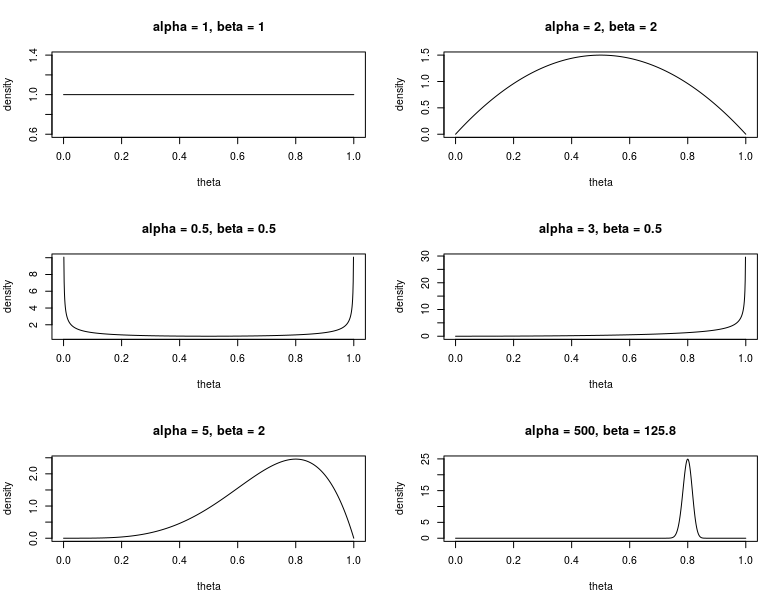
\includegraphics[height=0.85\textheight]{betaDistribution}
\end{figure}
\end{frame}

\begin{frame}
\frametitle{Beta-Verteilung}
\begin{itemize}
	\item<1-> $X\sim Bin(n,\theta)~,\quad \Theta\sim Be(\alpha,\beta)$
	\item<2-> $\Rightarrow f(\theta|x)\propto f(x|\theta)f(\theta)\propto \theta^x(1-\theta)^{n-x}\theta^{\alpha-1}(1-\theta)^{\beta-1}$
	\item<3-> $\Rightarrow \Theta|x \sim Be(\alpha+x,\beta+n-x)$
\end{itemize}
\end{frame}

\begin{frame}
\frametitle{Beta-Verteilung Beispiel}
\begin{columns}
	\uncover<1,2,3,4>{\begin{column}{0.5\textwidth}
		\begin{itemize}
			\item<1-> $\Theta\sim Be(3,2)~,\quad X\sim Bin(n,\theta)$
			\item<2-> Ergebnis der Stichprobe mit Umfang $n=10$: $x=8$
			\item<3-> $\Rightarrow \Theta|x\sim Be(11,4)$
		\end{itemize}
	\end{column}}
	\uncover<4>{\begin{column}{0.5\textwidth}
		\begin{figure}
			\begin{figure}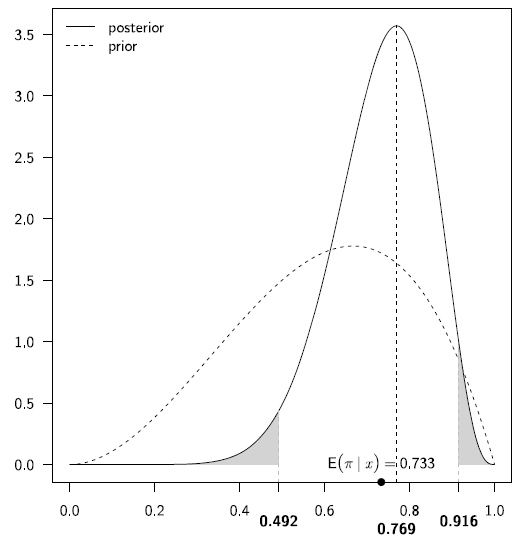
\includegraphics[width=0.75\textwidth]{beta}\caption{Held, Bov\'{e}: Applied Statistical Inference, S. 173}\end{figure}
		\end{figure}
	\end{column}}
\end{columns}
\end{frame}

\begin{frame}
\frametitle{Capture-Recapture-Method}
\begin{itemize}
	\item<1-> Möchte Anzahl $N$ von Fischen in einem See bestimmen
	\item<2-> Entnehme $M$ Fische, markiere diese und gebe sie wieder zurück
	\item<3-> Entnehme $n$ Fische und bestimme Anzahl $x$ der markierten Fische
	\item<4-> Naiver Ansatz: $\frac{M}{N}\approx \frac{x}{n}$
	\item<5-> Nachteil: Keine Information über Ungenauigkeit des Verfahrens
\end{itemize}
\end{frame}

\begin{frame}
\frametitle{Capture-Recapture-Method}
\begin{itemize}
	\item<1-> Ansatz mittels Bayesscher Inferenz:
	\item<2-> Likelihood: $$f(x|N)=\frac{\binom{M}{x}\binom{N-M}{n-x}}{\binom{N}{n}}$$
	\item<3-> Geometrische Verteilung als Prior: $f(N)\propto \pi(1-\pi)^{N-1}$
	\item<4-> Bsp.: $M=26\, ,~n=63\, ,~x=5\, ,~\pi=0,0011$
\end{itemize}
\end{frame}

\begin{frame}
\frametitle{Capture-Recapture-Method}
\begin{columns}
	\begin{column}{0.5\textwidth}
		\begin{figure}
			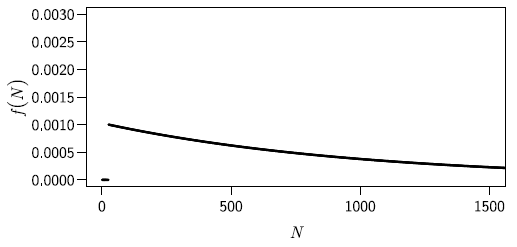
\includegraphics[width=0.9\textwidth]{geom}
			\caption{Held, Bov\'{e}: Applied Statistical Inference, S. 179}
		\end{figure}
	\end{column}
	\begin{column}{0.5\textwidth}
		\begin{figure}
			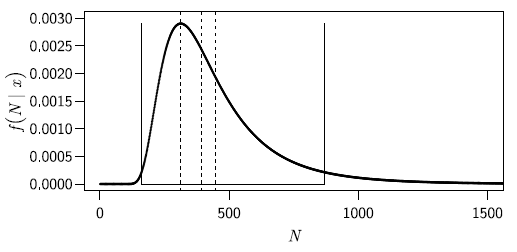
\includegraphics[width=0.9\textwidth]{capture-recapture}
			\caption{ebd.}
		\end{figure}
	\end{column}
\end{columns}
\begin{itemize}
	\item<1-> $Mod(N|x)=313\, ,~Med(N|x)=392\, ,~E(N|x)=446.5$
	\item<2-> $95\%$ HPD Intervall: $[61; 869]$
	\item<3-> Naiver Ansatz liefert: $N\approx 327,6$
\end{itemize}
\end{frame}

\begin{frame}
\frametitle{Conjugate prior distribution}
\begin{itemize}
	\item<1-> Eine Klasse $\mathscr{C}$ von Verteilungen heißt konjugiert zu $L(\theta)~(=f(x|\theta))$, wenn gilt: Aus $f(\theta)\in\mathscr{C}$ folgt $f(\theta|x)\in\mathscr{C}$.
	\item<2-> Beta-Verteilung ist konjugiert zur Binomialverteilung
	\item<3-> Normalverteilung (mit unbekanntem Erwartungswert) ist zu sich selbst konjugiert
\end{itemize}
\end{frame}

\begin{frame}
\frametitle{Uneigentliche Verteilungen}
\begin{itemize}
	\item<1-> Verteilung mit Dichtefunktion $f(\theta)$ heißt uneigentlich, falls $$\int_{\Theta}f(\theta)\,\text{d}\theta = \infty$$
	\item<2-> Kann dennoch eingesetzt werden, falls Posteriori Verteilung wohldefiniert ist
	\item<3-> Bsp.: Haldane's prior $Be(0,0)$
\end{itemize}
\end{frame}

\begin{frame}
\frametitle{Variablentransformation}
\begin{itemize}
	\item $Y=g(X)$
	\item $$f_Y(y)=f_X(g^{-1}(y))\left|\frac{\text{d}g^{-1}(y)}{\text{d}y}\right|$$
\end{itemize}
\end{frame}

\begin{frame}
\frametitle{Jeffrey's prior}
\begin{itemize}
	\item<1-> Ziel: Priori Verteilung invariant unter Variablentransformation
	\item<2-> Fisher Information: $$I(\theta)=-\frac{\text{d}^2l(\theta)}{\text{d}\theta^2}$$
	mit log-likelihood function $l(\theta)=ln(L(\theta))$
	\item<3-> Erwartete Fisher Information: $$J(\theta)=E(I(\theta;X))$$
	wobei der Erwartungswert bezüglich $X$ gebildet wird
	\item<4-> Jeffrey's prior $$f(\theta)\propto\sqrt{J(\theta)}$$
\end{itemize}
\end{frame}

\begin{frame}
\frametitle{Jeffrey's prior}
\uncover<1,2,3>{
\begin{itemize}
	\item<1-> Für multivariate Verteilungen: Erwartete Fisher Information Matrix $$[J(\boldsymbol{\theta})]_{ij}=E(-\partial_i\partial_jl(\boldsymbol{\theta}))$$
	\item<2-> Jeffrey's prior $$f(\boldsymbol{\theta})\propto\sqrt{\text{det}\,J(\boldsymbol{\theta})}$$
\end{itemize}}
\uncover<3>{\begin{satz}
	Jeffrey's prior ist invariant unter Variablentransformation, d.h. wenn $\phi = g(\theta)$ und $f_{\theta}(\theta)\propto \sqrt{J_{\theta}(\theta)}$, dann ist $f_{\phi}(\phi)\propto \sqrt{J_{\phi}(\phi)}$.
\end{satz}}
\end{frame}

\begin{frame}
\frametitle{Jeffrey's prior für $Bin(n,\theta)$}
\begin{itemize}
	\item<1-> $X\sim Bin(n,\theta)$, also $f(x|\theta)= \binom{n}{x}\theta^x(1-\theta)^{n-x}$
	\item<2-> $l(\theta)=x\,ln(\theta)+(n-x)\,ln(1-\theta)+const$
	\item<3-> $-\frac{\text{d}^2l(\theta)}{\text{d}\theta^2}=\frac{x}{\theta^2}-\frac{n-x}{(1-\theta)^2}$ 
	\item<4-> $E(-\frac{\text{d}^2l(\theta)}{\text{d}\theta^2}) = \frac{n\theta}{\theta^2}-\frac{n(1-\theta)}{(1-\theta)^2}=\frac{n}{\theta(1-\theta)}$
	\item<5-> $\Rightarrow \sqrt{J(\theta)}\propto Be(\frac{1}{2},\frac{1}{2})$
\end{itemize}
\end{frame}

\begin{frame}
\frametitle{Jeffrey's prior für Multinomialverteilung}
\begin{itemize}
	\item<1-> $\boldsymbol{x}=(x_1,\dots,x_p)\,,~\boldsymbol{\theta}=(\theta_1,\dots,\theta_p)$ mit $\sum_{i=1}^p\theta_p = 1$
	\item<2-> Multinomialverteilung $M_p(n,\boldsymbol{\theta})$: $$f(\boldsymbol{x})=\left\{\begin{array}{ll}
	\frac{n!}{\prod_{i=1}^{p}x_i!}\prod_{i=1}^{p}\theta_i^{x_i} & \text{falls }\sum_{i=1}^{p}x_i=n\\
	0 & \text{sonst}
	\end{array}\right.$$
	\item<3-> Dirichlet-Verteilung $D(\alpha_1,\dots,\alpha_p)$: $$f(\boldsymbol{\theta})\propto\prod_{i=1}^{p}\theta_i^{\alpha_i-1}$$
	\item<4-> Jeffrey's prior für $M_p(n,\boldsymbol{\theta})$:
	$$\boldsymbol{\theta}\sim D\left(\frac{1}{2},\dots,\frac{1}{2}\right)$$
\end{itemize}
\end{frame}

\begin{frame}
\frametitle{Asymptotisches Verhalten}
\begin{itemize}
	\item<1-> Parametermenge $\Theta=\{\theta_0,\theta_1,\dots\}$, $\theta_0$ ist wahrer Parameter, $X_{1:n}$ Stichprobe von Verteilung mit Dichtefunktion $f(x|\theta)\,,\,\theta\in\Theta$. Dann gilt:
	$$\underset{n\rightarrow\infty}{\text{lim}}f(\theta_0|x_{1:n})=1\quad \text{und}\quad \underset{n\rightarrow\infty}{\text{lim}}f(\theta_i|x_{1:n})=0~\forall i\neq 0$$
\end{itemize}
\end{frame}

\begin{frame}
\frametitle{Empirische Bayes Methoden}
\begin{itemize}
	\item<1-> Wählen Priori Verteilung in Abhängigkeit von erhaltenen Daten
	\item<2-> Bsp.: Analyse der Trefferquoten von Baseballspielern:
	\item<3-> Spieler A hat 4 von 10 Bällen getroffen, Spieler B hat 300 von 1000 Bällen getroffen. Welcher Spieler ist besser?
	\item<4-> Trefferzahl $X\sim Bin(n,\theta)$, Treffwahrscheinlichkeit $\theta\sim Be(\alpha,\beta)$
\end{itemize}
\end{frame}

\begin{frame}
\frametitle{Empirische Bayes Methoden}
\begin{columns}
	\uncover<1,2,3,4,5>{\begin{column}{0.6\textwidth}
		\begin{itemize}
			\item<1-> Bilde Priori Verteilung durch Interpolation über Werte aller Baseballspieler
			\item<3-> $\Rightarrow \theta\sim Be(78,661\,;\,224,875)$
			\item<4-> Posteriori Trefferverteilung für Spieler A: $\theta|x\sim Be(82,661\,;\,230,875)$ hat Erwartungswert 0,264
			\item<5-> Posteriori Trefferverteilung für Spieler B: $\theta|x\sim Be(378,661\,;\,924,875)$ hat Erwartungswert 0,29
		\end{itemize}
	\end{column}}
	\uncover<2,3,4,5>{\begin{column}{0.4\textwidth}
		\begin{figure}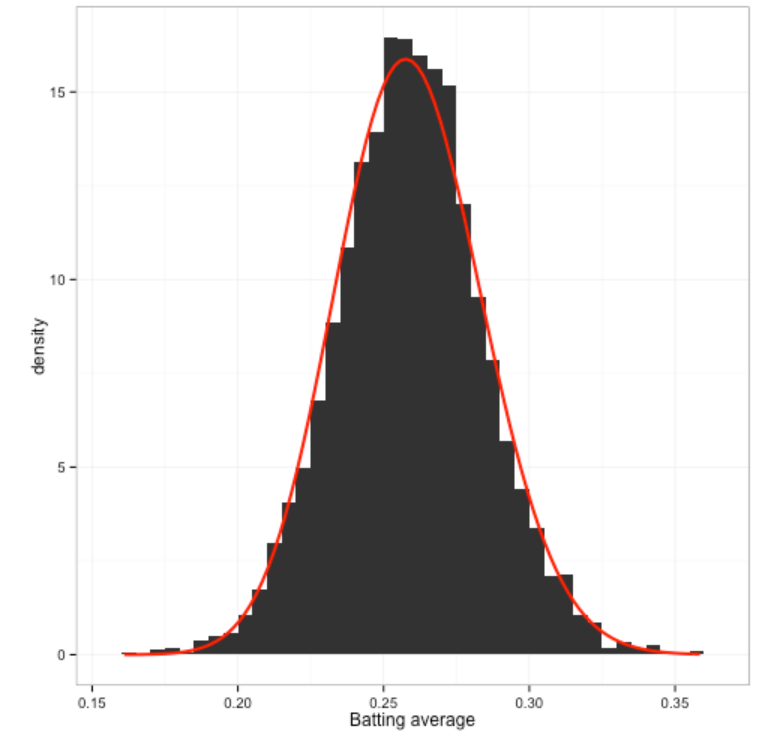
\includegraphics[width=\textwidth]{baseball}\caption{varianceexplained.org}\end{figure}
	\end{column}}
\end{columns}
\end{frame}

\section{Bibliographie}
\begin{frame}
\frametitle{Bibliographie}
\begin{itemize}
	\item Held, Bov\'{e}: Applied Statistical Inference
\end{itemize}
\end{frame}

\end{document}
